\section{Empirical Evaluation} \label{sec:evaluation}

The typical approach to identifying specific classes on online users relies on expert-generated ground truth, i.e., to determine which users belong to the desired class. 
Such approach, however, is vulnerable to  the subjectivity of the experts, whereby the evalution would  be measuring the fit of the model to the specific experts' own opinion. 
In contrast, we follow an \textit{unsupervised} approach where there is no a priori knowledge of user relevance.  
In this section we aim to demonstrate the value of our pipeline in creating a database of online profiles, which are pre-selected according to specific topological properties in order to filter out background noise,  along with a community-accepted set of engineered features that are ready to be mined using any user-defined function.
%
Thus, our evaluation (i) shows the pipeline in action on a significant set of 25 initial contexts, and (ii) demonstrates useful ranking functions that operate on the resulting database, aimed at capturing the empirical notion of  \textit{online activists}.
% We  start by manually selecting initial  contexts from a single social domain, namely public healthcare campaigns in the UK, to demonstrate network construction, breakdown of each  context network into communities, and harvesting of users from each community, along with their metrics.
% We then provide examples of ranking functions .

The pipeline is fully implemented in Python using Pandas and the NetworkX and Selenium public libraries and is available on github\footnote{Twitter Network Analysis repository: \url{https://github.com/flaprimo/twitter-network-analysis}}. 
All experiments are performed on a single Azure node with standard commodity configuration.
Note that we do not focus on system performance as all components operate in near-real time. One exception is  Twitter content harvesting, which is limited by the Twitter API and requires approximately 2 hours per context.

\subsection{Contexts and networks} \label{sec:contexts}
 
We have manually selected 25 contexts within the scope of health awareness campaigns in the UK, all occurring in 2018 and well-characterised using predefined hashtags.
Due to limitations imposed by Twitter on the number of posts that can be retrieved within a time interval, only $200$ tweets were retrieved from each context.
 Table~\ref{tab:contexts} lists the events along with key metrics for their corresponding user-user networks. 
To recall, \textit{assortativity} measures how frequently nodes are likely to connect to other nodes with the same degree ($>0$) or with a different degree ($<0$). 
Negative figures (mean: -0.22, std dev: 0.17) are in line with what is observed on the broader Twitter network~\cite{Fisher2017}.
%
The very small figures for density (mean: 0.004, std dev: 0.002), defined as $\frac{\#edges }{\mathit{\mathit{\#nodes}} \cdot (\mathit{\#nodes} -1)}$, suggest very few connections exist amongst users within a context. 
This makes it difficult to detect meaningful communities, as described below, thus for some context the topological metrics are measured on the entire network as opposed to within each community.
This view is also supported by the average node degree (mean: 2.04, std dev: 0.46) and the ratio of strongly connected components to the number of nodes (mean: 0.98, std. dev. 0.02).

\begin{table}
	\resizebox{\textwidth}{!}{
	    \begin{tabularx}{\textwidth}{|X|P{2.2cm}|P{1.2cm}|P{1cm}|P{1.4cm}|P{1.2cm}|P{1.3cm}|}

\hline
\textbf{Context name} & \textbf{Period (2018)} & \textbf{Nodes} & \textbf{Edges} & \textbf{Density} & \textbf{Avg degree} & \textbf{Assor-tativity} \\ \hline
16 days of action & 11-25 / 12-10 & 396 & 349 & 0.002 & 1.8 & -0.1 \\ \hline
Elf day & 12-03 / 12-12 & 365 & 436 & 0.003 & 2.4 & -0.2 \\ \hline
Dry january & 01-01 / 01-31 & 235 & 234 & 0.004 & 2.0 & -0.3 \\ \hline
Cervical cancer prevention week & 01-21 / 01-27 & 209 & 192 & 0.004 & 1.8 & -0.1 \\ \hline
Time to talk day & 02-06 / 02-07 & 268 & 231 & 0.003 & 1.7 & -0.2 \\ \hline
Eating disorder awareness week & 02-25 / 03-03 & 256 & 241 & 0.004 & 1.9 & -0.2 \\ \hline
Rare disease day & 02-28 / 03-01 & 294 & 206 & 0.002 & 1.4 & -0.2 \\ \hline
Ovarian cancer awareness month & 03-01 / 03-31 & 215 & 202 & 0.004 & 1.9 & -0.4 \\ \hline
Nutrition and hydration week & 03-11 / 03-17 & 273 & 326 & 0.004 & 2.4 & -0.3 \\ \hline
Brain awareness week & 03-11 / 03-17 & 307 & 281 & 0.003 & 1.8 & -0.1 \\ \hline
No smoking day & 03-13 / 03-14 & 254 & 219 & 0.003 & 1.7 & -0.3 \\ \hline
Epilepsy awareness purple day & 03-26 / 03-27 & 306 & 252 & 0.003 & 1.6 & -0.2 \\ \hline
Experience of care week & 04-23 / 04-27 & 176 & 196 & 0.006 & 2.2 & -0.1 \\ \hline
Brain injury week & 05-01 / 05-31 & 238 & 306 & 0.005 & 2.6 & -0.1 \\ \hline
Mental health awareness week & 05-14 / 05-20 & 268 & 245 & 0.003 & 1.8 & -0.5 \\ \hline
Dementia action week & 05-21 / 05-31 & 300 & 300 & 0.003 & 2.0 & -0.0 \\ \hline
Mnd awareness month & 06-01 / 06-30 & 141 & 234 & 0.012 & 3.3 & -0.3 \\ \hline
Wear purple for jia & 06-01 / 06-30 & 165 & 245 & 0.009 & 3.0 & -0.5 \\ \hline
Carers week & 06-11 / 06-17 & 270 & 277 & 0.004 & 2.1 & 0.0 \\ \hline
National dementia carers & 09-09 / 09-10 & 184 & 177 & 0.005 & 1.9 & -0.2 \\ \hline
Mens health week & 06-11 / 06-17 & 264 & 214 & 0.003 & 1.6 & -0.2 \\ \hline
Stress awareness day & 11-07 / 11-08 & 293 & 209 & 0.002 & 1.4 & -0.2 \\ \hline
National dyslexia week & 10-01 / 10-07 & 229 & 235 & 0.004 & 2.1 & -0.2 \\ \hline
Ocd awareness week & 10-07 / 10-13 & 202 & 193 & 0.005 & 1.9 & -0.6 \\ \hline
Jeans for genes day & 09-21 / 09-22 & 246 & 325 & 0.005 & 2.6 & -0.2 \\ \hline

\end{tabularx}

	}
	\caption{List of contexts used in the experiments along with network metrics.}
	\label{tab:contexts}
\end{table}

\subsection{Communities}  \label{sec:communities}

 \demon~and \infomap~ produce significantly different communities in each network. 
%
Specifically, \demon~identifies communities in only 48\% of the netnworks.
For these, only the users who belong to one of those community are added. 
These are about 6\% of the users on average, with an average of only 1.92 communities per network.

For the remaining 52\% of networks where no communities are detected, users' in-degrees are calculated using the entire network, and all users in the network are added to the database.
%
When using \demon, 3,570 users being added to the database.
The average assortativity of individual \demon~communities is slightly negative -0.28, in line with the average for their parent networks.

In contrast, \infomap~provides meaningful communities for all networks.
Those with fewer than 3 users are discarded, leaving  18.88 communities per network on average, with 8.5 users per community on average.
% The rightmost column in Table~\ref{tab:contexts} reports the number of communities normalised by the size of the network, where a  contains . 
When using Infomap, 3,567 users were added to the database (on average 253 users per network).
The average assortativity across all communities is again slightly negative (-0.43).
%
Table~\ref{tab:demon-vs-infomap} compares the two approaches on the key metrics just discussed. On the basis of this comparison, we have chosen Infomap for  our implementation and evaluation.

\begin{table}
	\resizebox{\textwidth}{!}{
	    \begin{tabularx}{\textwidth}{|X|P{1.7cm}|P{1.7cm}|}
\hline
\textbf{Metric} & \textbf{\demon} & \textbf{\infomap} \\ \hline
Fraction of networks with null communities & 0.52 & 0.0 \\ \hline
Number of communities per context (avg) & 1.92 & 18.88 \\ \hline
Fraction of network users added to the DB  (avg) & 0.06 & 0.59 \\ \hline
Fraction of repeat users  added to the DB across networks & 0.28 & 0.37 \\ \hline
\end{tabularx}
	}
	\caption{Comparing \demon~to \infomap~for community detection.}
	\label{tab:demon-vs-infomap}
\end{table}

\subsection{Users discovery}  \label{sec:users}

Repeat users, those who appear in multiple contexts, are particularly interesting as they provide a stronger signal. 
Out of the total 3,567, 160 users  appear at least in two of the 25 contexts.
After community detection, only 61 of these users are still seen as repeat users,
while the remaining 99 are either removed altogether, or they only appear once.
Of these, 55 appear twice, 2 appear three times, and 2 appear four times. 
Thus, only 1.6\% of users appear more than once when communities with more than 3 users are considered, compared to the overall 4.5\% repeat users.
%
Table~\ref{tab:repeat-users} reports the top repeat users along with their \textit{Follower Rank}.  \anote{FLAVIO: Apart from jeremy\_hunt, which is a politician, and colesmillerllp, which is a legal firm, the rest are associations and foundations related with healthcare. This is expected as the table is sorted for "Participations" and subsequently by "Follower Rank". This can be interpreted as the organizers of NHS social media campaigns are associations and foundations related to the NHS.}
Recall that the Follower Rank $FR$ is usually taken as an indication of how ``popularity''. 
Interesting users are therefore the repeat users with a low $FR$  (it is not surprising to see Mr. Hunt, who at the time of the events was Secretary of State for Health and Social Care in the UK, with $FR =1.$
%
Fig.~\ref{fig:repeat-users-frequency} shows the number of repeat users per context. 

\begin{table}
	\centering
	\resizebox{\textwidth}{!}{
		\begin{tabularx}{\textwidth}{|p{2.5cm}|X|P{2.4cm}|P{2.4cm}|}
\hline
\textbf{Username} & \textbf{Name} & \textbf{Follower rank} & \textbf{Participations} \\ \hline
alzheimerssoc & Alzheimer's Society & 0.99 & 4 \\ \hline
dementiauk & Dementia UK & 0.98 & 4 \\ \hline
mentalhealth & Mental Health Fdn & 0.97 & 3 \\ \hline
colesmillerllp & Coles Miller LLP & 0.65 & 3 \\ \hline
rdash\_nhs & RDaSH NHS FT & 0.88 & 2 \\ \hline
alzsocseengland & Alzheimer's Society - South ... & 0.64 & 2 \\ \hline
jeremy\_hunt & Jeremy Hunt & 1.0 & 2 \\ \hline
nhsengland & NHS England & 0.99 & 2 \\ \hline
carersuk & Carers UK & 0.95 & 2 \\ \hline
mndassoc & MND Association & 0.64 & 2 \\ \hline
\end{tabularx}
	}
	\caption{Top-10 repeat users, amongst those identified as belonging to some community.}
	\label{tab:repeat-users}
\end{table}

\begin{figure*}
	\centering
	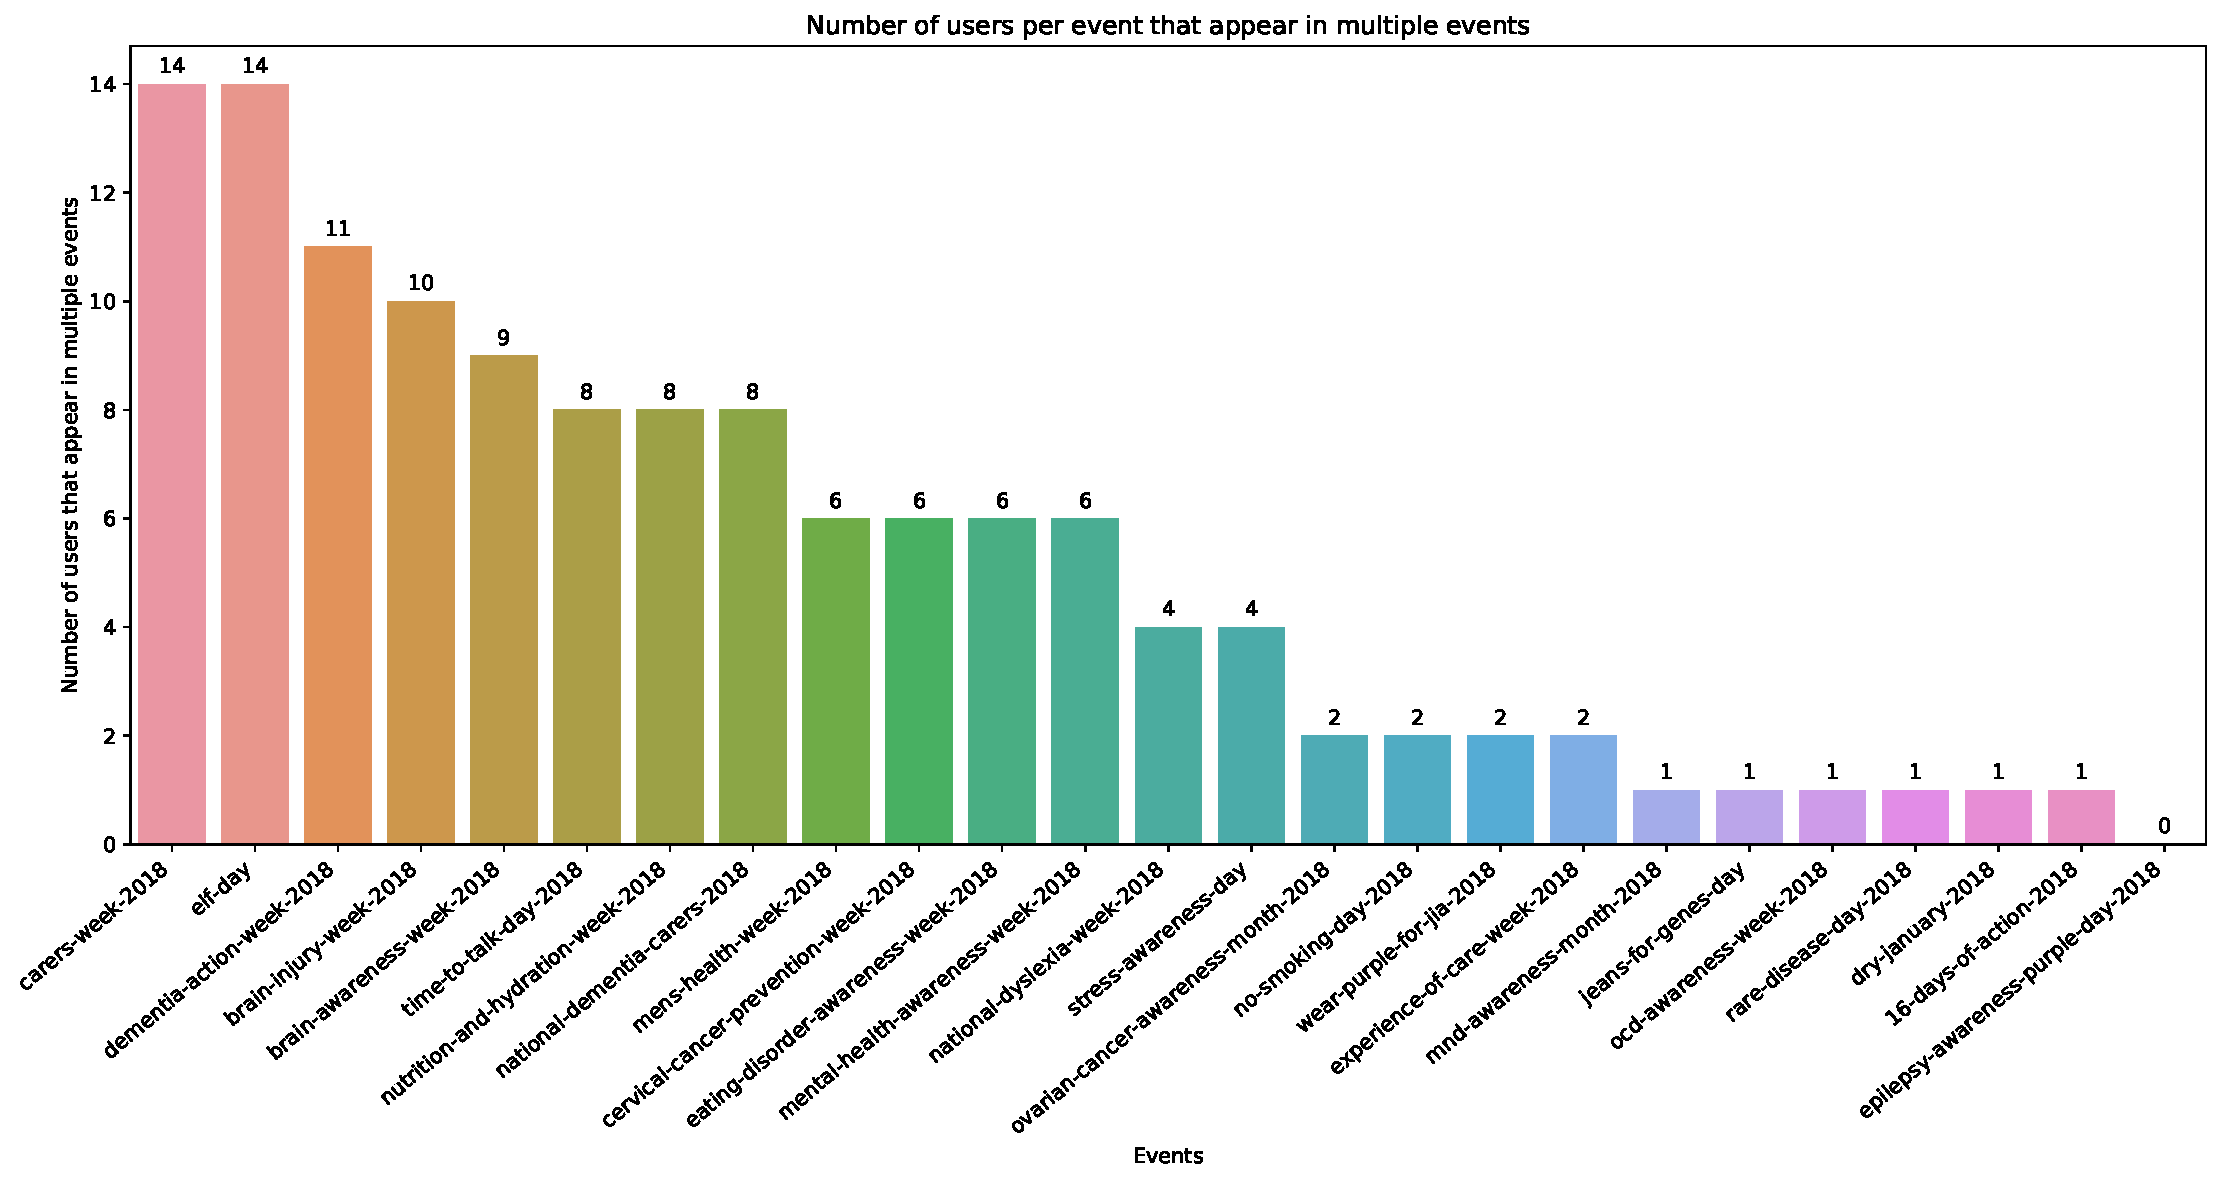
\includegraphics[width=\textwidth]{figures/repeat-users-frequency}
	\caption{Number of repeat users for each context}
	\label{fig:repeat-users-frequency}
\end{figure*}

\subsection{Users ranking} \label{sec:ranking}

Once the database is populated, 2 ranking functions are tested against it.
%
\begin{table}
	\centering
	\resizebox{\textwidth}{!}{
		\begin{tabular}{P{0.6cm}|p{2.4cm}|p{1.6cm}|p{2.4cm}|p{2.4cm}|p{1.6cm}|p{2.4cm}|}

\cline{2-7}
\multicolumn{1}{l|}{} & \multicolumn{3}{c|}{\textbf{Rank 1}} & \multicolumn{3}{c|}{\textbf{Rank 2}} \\ \hline
\multicolumn{1}{|c|}{\textbf{\#}} & \textbf{User} & \textbf{Type} & \textbf{Description} & \textbf{User} & \textbf{Type} & \textbf{Description} \\ \hline
\multicolumn{1}{|c|}{1} & homesnutrition & in-topic association & Promote examples of good nutrition in nursing homes & johnneustadt & in-topic individual & Naturopathic physician which is very active in NHS related events \\ \hline
\multicolumn{1}{|c|}{2} & ficajones & in-topic individual & Ward manager & jo\_millar27 & in-topic individual & Ordinary person that mostly retweets NHS related news \\ \hline
\multicolumn{1}{|c|}{3} & helenvweaver & in-topic individual & Neuro physiotherapist & hatchbrenner & off-topic association & Legal advice \\ \hline
\multicolumn{1}{|c|}{4} & spriggsnutri & in-topic association & Nutritional therapy & nchawkes & in-topic individual & Consultant Clinical Psychologist in Eating Disorders \\ \hline
\multicolumn{1}{|c|}{5} & critcarelthtr & in-topic association & Critical care in Preston & moz0373runner & in-topic individual & Fundraiser for NHS related events \\ \hline
\multicolumn{1}{|c|}{6} & danielleroisin\_ & in-topic individual & Ordinary person that mostly retweets NHS related news & aimsonhealth & in-topic individual & Health student which has a website and social account pages dedicated to NHS topics \\ \hline
\multicolumn{1}{|c|}{7} & mynameisandyj & in-topic individual & Ordinary person dedicated to NHS, patients care and staff & wordsharkv5 & off-topic individual & Educational software house for children \\ \hline
\multicolumn{1}{|c|}{8} & fionaliu92 & in-topic individual & Dietitian & fullcircle\_play & in-topic association & Theatre play related to mental health \\ \hline
\multicolumn{1}{|c|}{9} & ldpartnership & in-topic association & Community diabetes team that provides diabetes care & qsprivatehealth & in-topic association & Private healthcare \\ \hline
\multicolumn{1}{|c|}{10} & milaestevam1 & off-topic individual & Ordinary person & socialissp & off-topic association & Interdisciplinay virtual platform for general knowlwdge \\ \hline

\end{tabular}
	}
	\caption{Top-10 ranked users for rank 1 and rank 2.}
	\label{tab:rank1}
\end{table}
%
\begin{align}
\textit{Rank 1:} ~ \mathit{R1}(u) & = \frac{1}{\sum_{u \in C} \mathit{IC}(u) + 1} \cdot \sum_{u \in C} \mathit{TF}(u) \label{eq:rank1} \\
\textit{Rank 2:} ~ \mathit{R2}(u) & = \lvert \mathit{FR}(u) - 1 \rvert \cdot \left(\sum_{u \in C} \mathit{TA}(U) + \sum_{u \in C} \mathit{IC}(U)\right) \label{eq:rank1}
\end{align}
%
Rank 1 assigns an higher scores to users which are at the margins of communities while giving credit to generic on-topic activities during the contexts.

Rank 2 penalises instead the popularity of the users, while awarding for prominence inside communities and information spreading by also considering shared links.

Rank 1 seems to favour more on-topic users (90\% for Rank 1 and 70\% for Rank 2). While Rank 2 seems to favour more, among in-topic users, individuals (55\% for Rank 1 and 71\% for Rank 2). 

Both ranks mostly show on-topic users (9 out of 10 for Rank 1 and 7 out of 10 for Rank 2). Rank 1 5/4 Rank 1 5/2 Rank 2

In both ranks users which participated to more than one context are rewarded. Users with $\mathit{FR}(u) = 0$ and $\mathit{min\_max(\lvert Tweets \rvert(u)) < 0.005}$ are considered not active and have been assigned lowest score.